\section{Design Model}

%%%%%%%%%%%%%%%%%%%%%%%%%%%%%%%%%%%%%%%
\subsection{Components and Overall Structure}
\label{sec:components}

In this section we show the overal structure of the design. The design is going
to be implemented in Java and Jess. The inference knowledge and domain knowledge
is mostly in the Jess part, while the task knowledge and user interaction is in
the Java part.

The modular structure can be seen in figure~\ref{fig:dm:modules}. The main
applicaton is implemented in Java with a model-view-controller design, see
section~\ref{sec:app}. The model part starts a Jess engine and loads facts and
rules that implement the system model and inferences over it.

In the working memory of the Jess engine are the domain rules, Jess facts
that represent inferential knowledge of car, and the domain parts, Jess facts
with knowledge about the current status of parts of the car.
Domain rules are not modified over a run of the program, while domain parts are modified. 

Information from the Java application goes to Jess by asserting support facts,
these are then interpeted as modifications of domain parts by support rules.
Information from Jess goes to the Java application by Jess queries made by that
application. 

The components in Jess are divided between a engine and a domain part. The
domain parts consists of the domain rules and the domain parts, these are implementations
of templates supplied by the engine. The engines Jess rules do forward and
backward reasoning on these domain rules and domain parts, see section \ref{sec:inferences}.
The domain rules and domain parts can be substituted by rules and parts from a
different domain while keeping the engine. The rules might be understandable by an
expert or user, as our car repair hobbyist does. The complexity of the inferences
made by the engine are not visible in the domain part.

\begin{figure}[htbp]
    \centering
    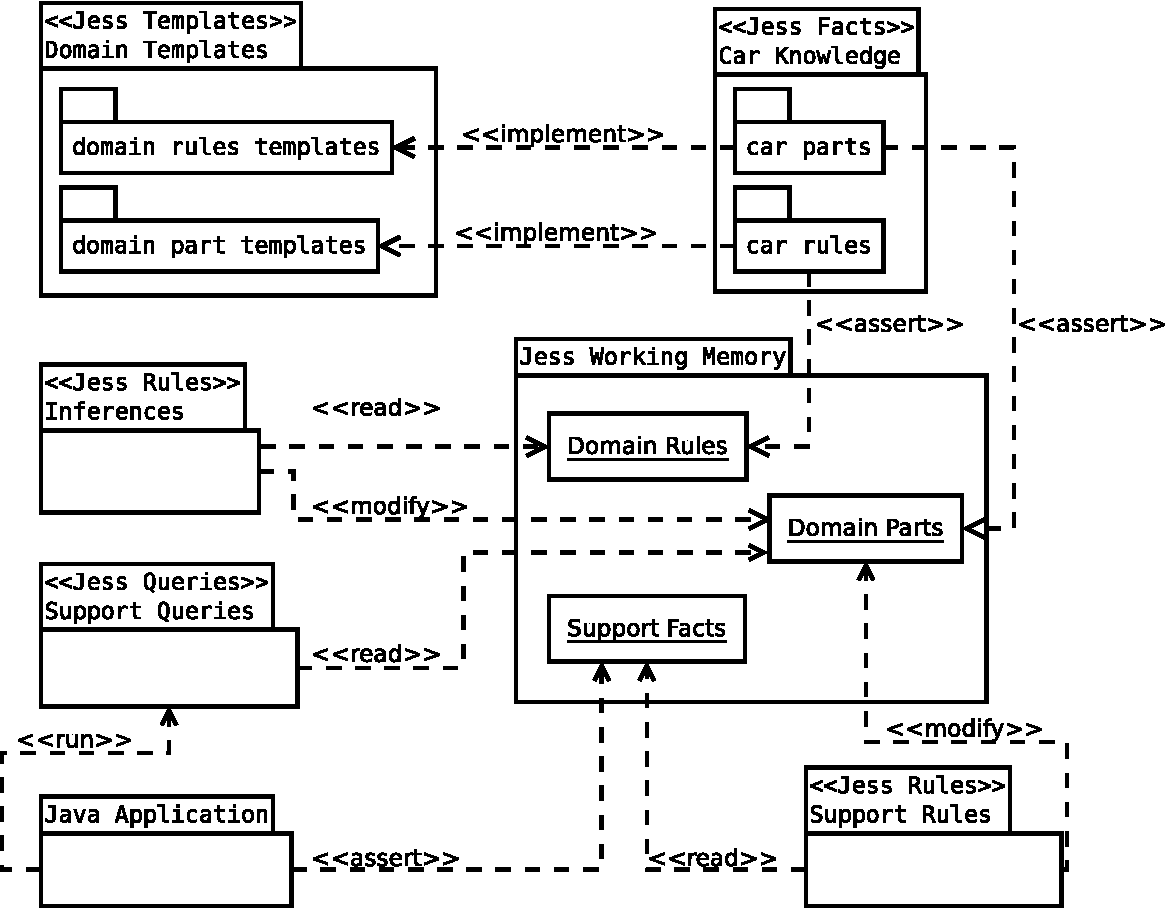
\includegraphics[width=1.00\textwidth]{dm-modules}
    \caption{The modular structure of the design model}
    \label{fig:dm:modules}
\end{figure}

%%%%%%%%%%%%%%%%%%%%%%%%%%%%%%%%%%%%%%%
\subsection{The process flow}
\label{sec:flow}

The overall flow of the application can be seen in the activity diagram in
figure~\ref{fig:dm:activity diagram}. It implements the communication, as
modelled in figure~\ref{fig:communicationPlan}, and the task method, as seen in
figure~\ref{fig:taskMethod}.

The process start when a complaint is reported to the system. The system then covers
all hypothesis that follow from the complaint. The rest of the process is one
big loop. It has two exits, when a succesfull repair is made, and when there are
no viable hypothesis left. Inside the loop, first, a hypothesis is selected with
user assistance. Secondly an attempt is made to make an observation. This is a
loop where the user is asked to observe all the possible observables on after
another. If the user want do do an observation the result is used to update the
hypothesis in the verify activity. If the user doesn't want do to any of the
observations or there are no observables for the hypothesis, the user is asked
to repair his or her car. If this repair is succesfull the problem is solved and
the program exits. If the repair isn't succesfull, the hypothesis is deemed
impossible by the system.

\begin{figure}[htbp]
    \centering
    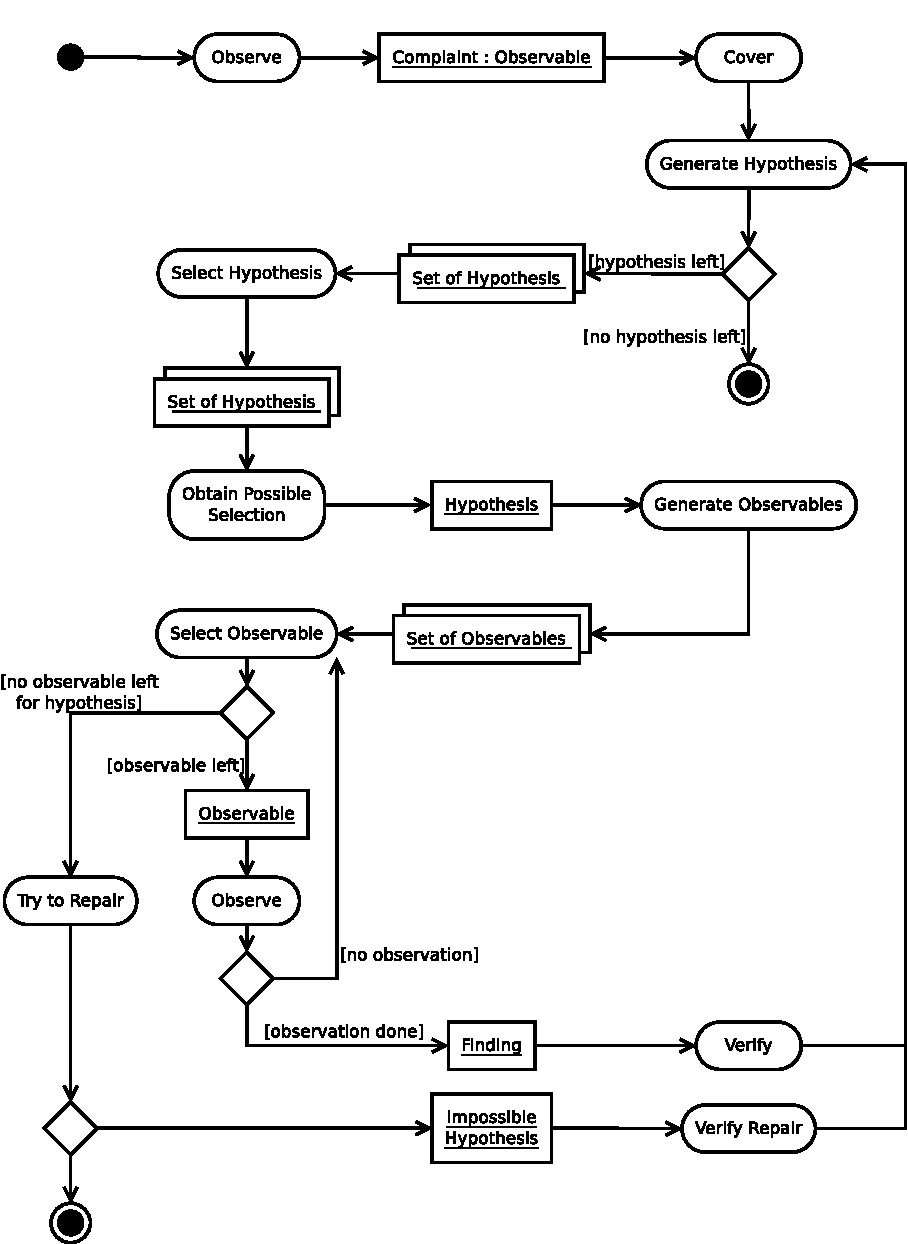
\includegraphics[width=1.00\textwidth]{dm-activity}
    \caption{The overal activity diagram of the application}
    \label{fig:dm:activity diagram}
\end{figure}

%%%%%%%%%%%%%%%%%%%%%%%%%%%%%%%%%%%%%%%
\subsection{The application}
\label{sec:app}

class diagram in figure~\ref{fig:dm:class diagram}. %TODO
\begin{figure}[htbp]
    \centering
    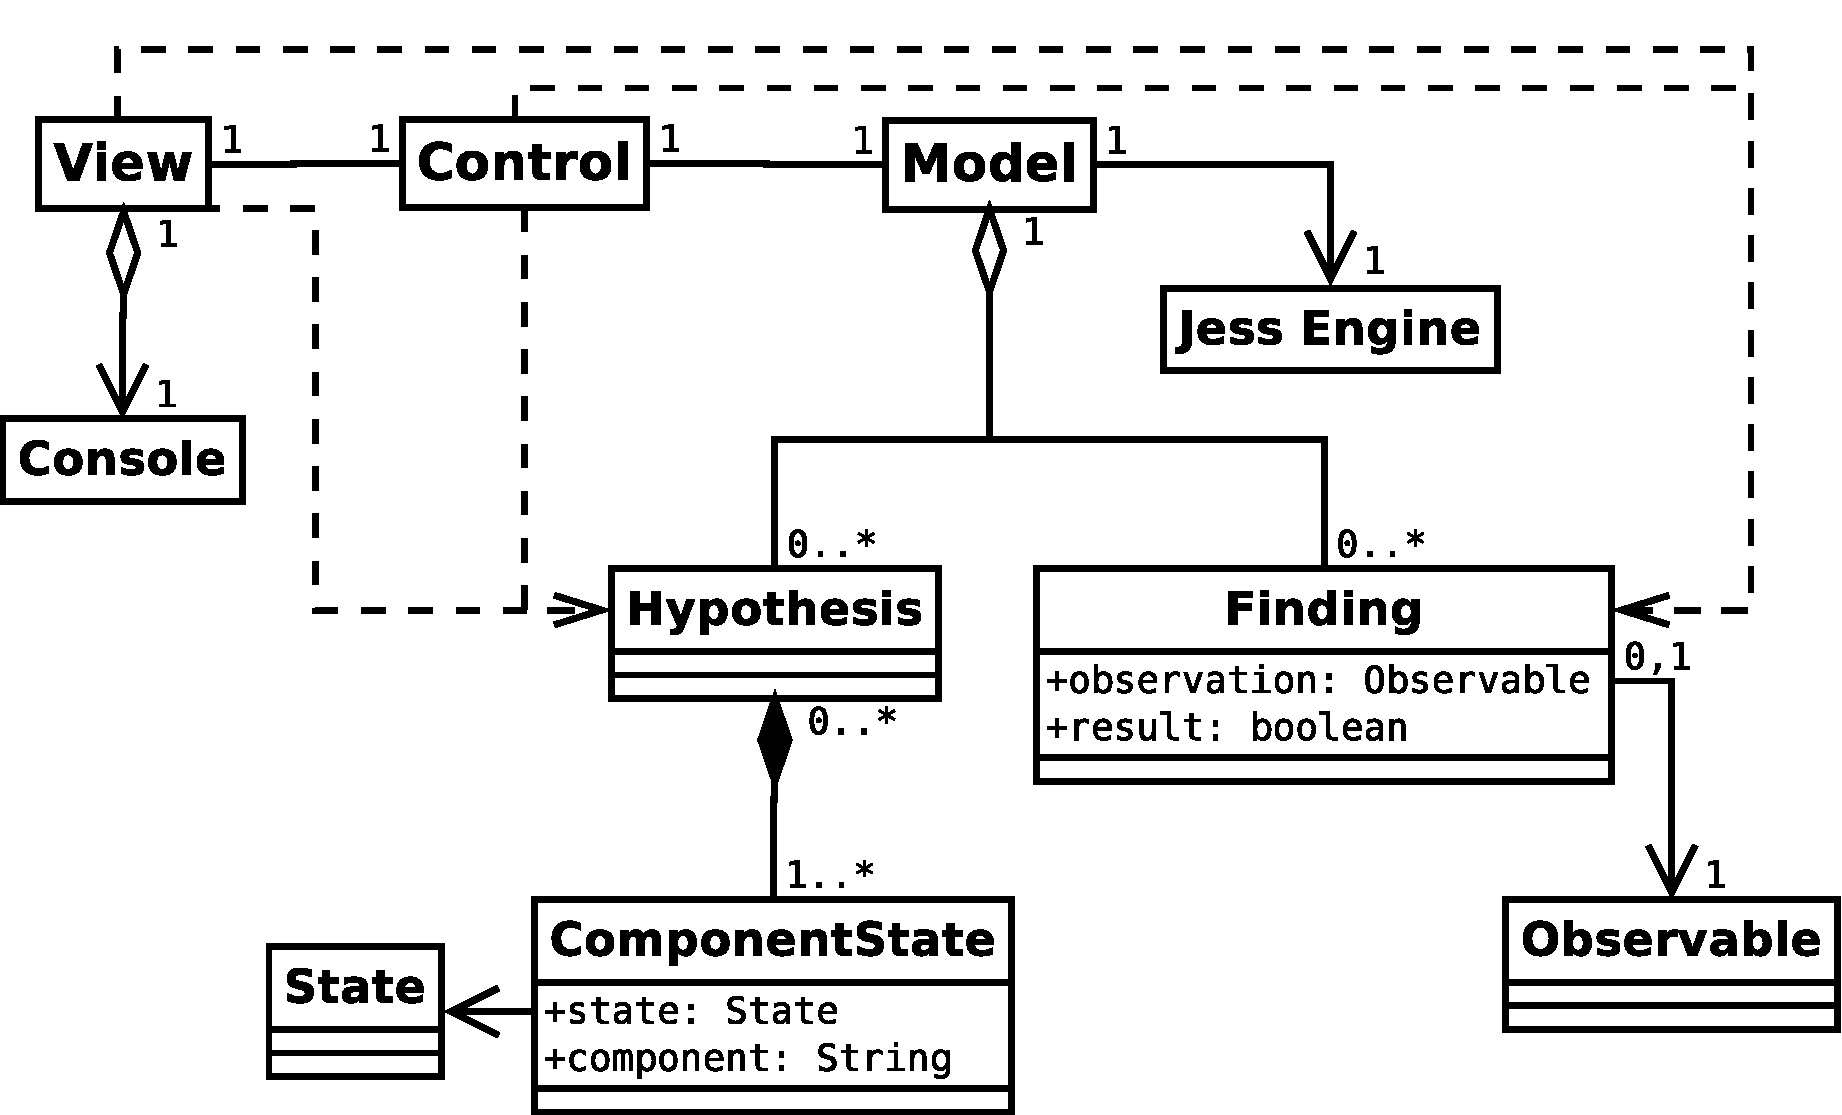
\includegraphics[width=1.00\textwidth]{dm-class}
    \caption{The class diagram of the Java application}
    \label{fig:dm:class diagram}
\end{figure}

The model-view-controller pattern is applied. The model keeps all the knowledge
of the system. The Java class is partly an interface to the part of the model
that is implemented in Jess and partly implements the knowledge of the model
itself, as explained in the next section. The control manages the process flow,
as described in the previous section, and communicates with the model and the
view components. The view implements the user interface and the part of the user
interaction that doesn't involve the model.

The activity diagram of figure~\ref{fig:dm:activity diagram} is further detailed
in three state diagrams showing the communication between the model, view and
controller components. The first diagram, in figure~\ref{fig:dm:sd cover}, %TODO
The second diagram, in figure~\ref{fig:dm:sd select}, %TODO
The third diagram, in figure~\ref{fig:dm:sd observe}, %TODO

\begin{figure}[htbp]
    \centering
    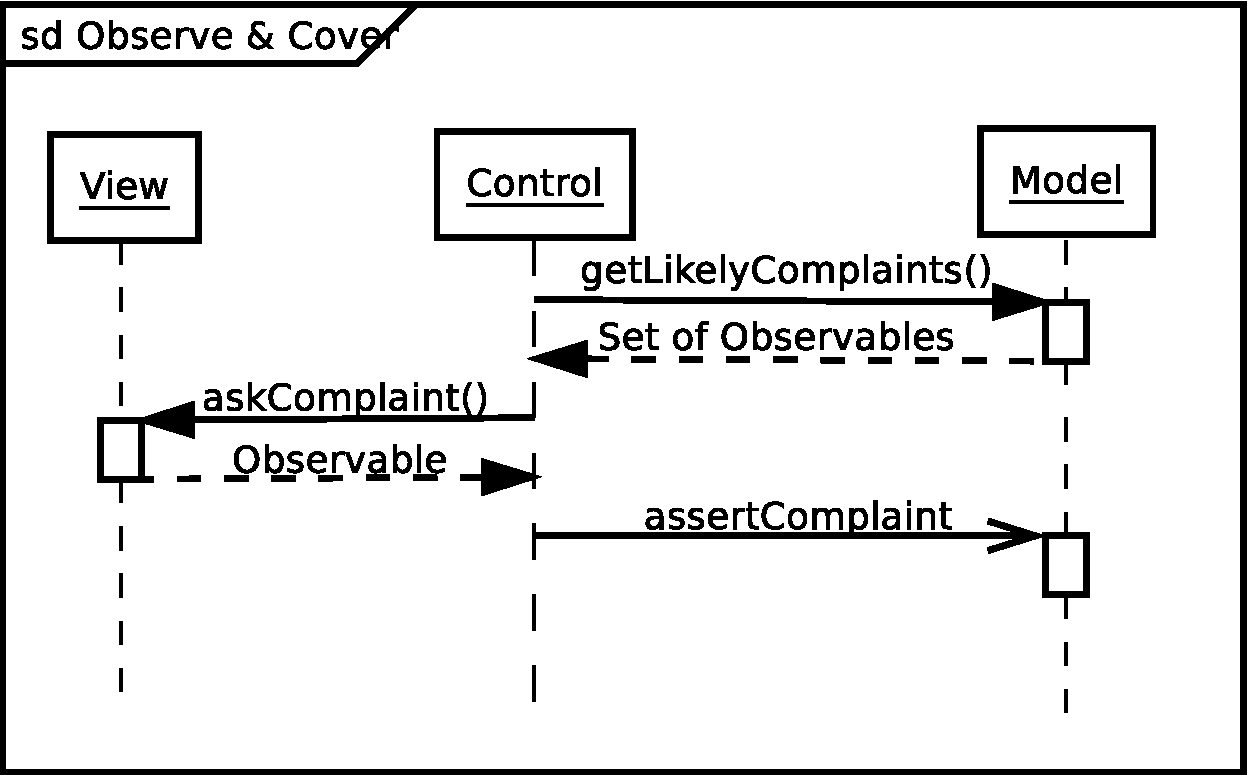
\includegraphics[width=1.00\textwidth]{dm-sd-cover}
    \caption{The state diagram detailing report and cover}
    \label{fig:dm:sd cover}
\end{figure}

\begin{figure}[htbp]
    \centering
    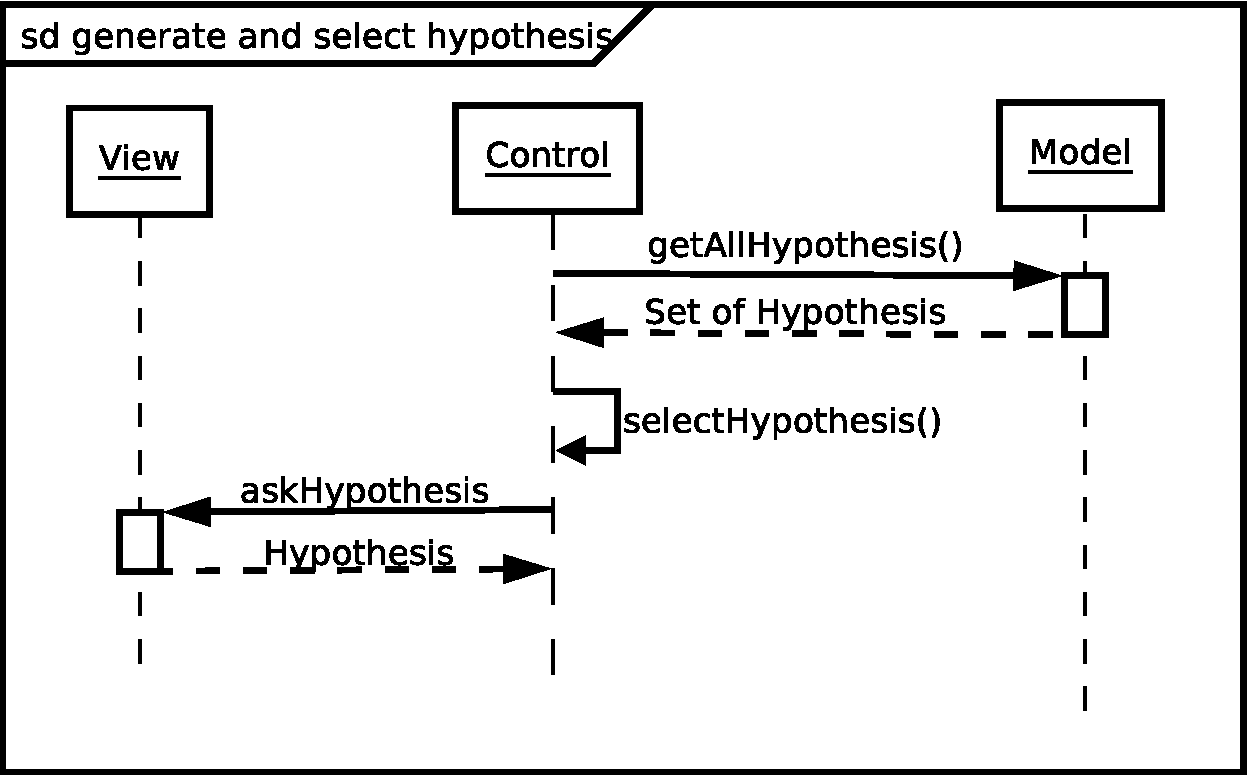
\includegraphics[width=1.00\textwidth]{dm-sd-select}
    \caption{The state diagram detailing generating and selecting hypothesis}
    \label{fig:dm:sd select}
\end{figure}

\begin{figure}[htbp]
    \centering
    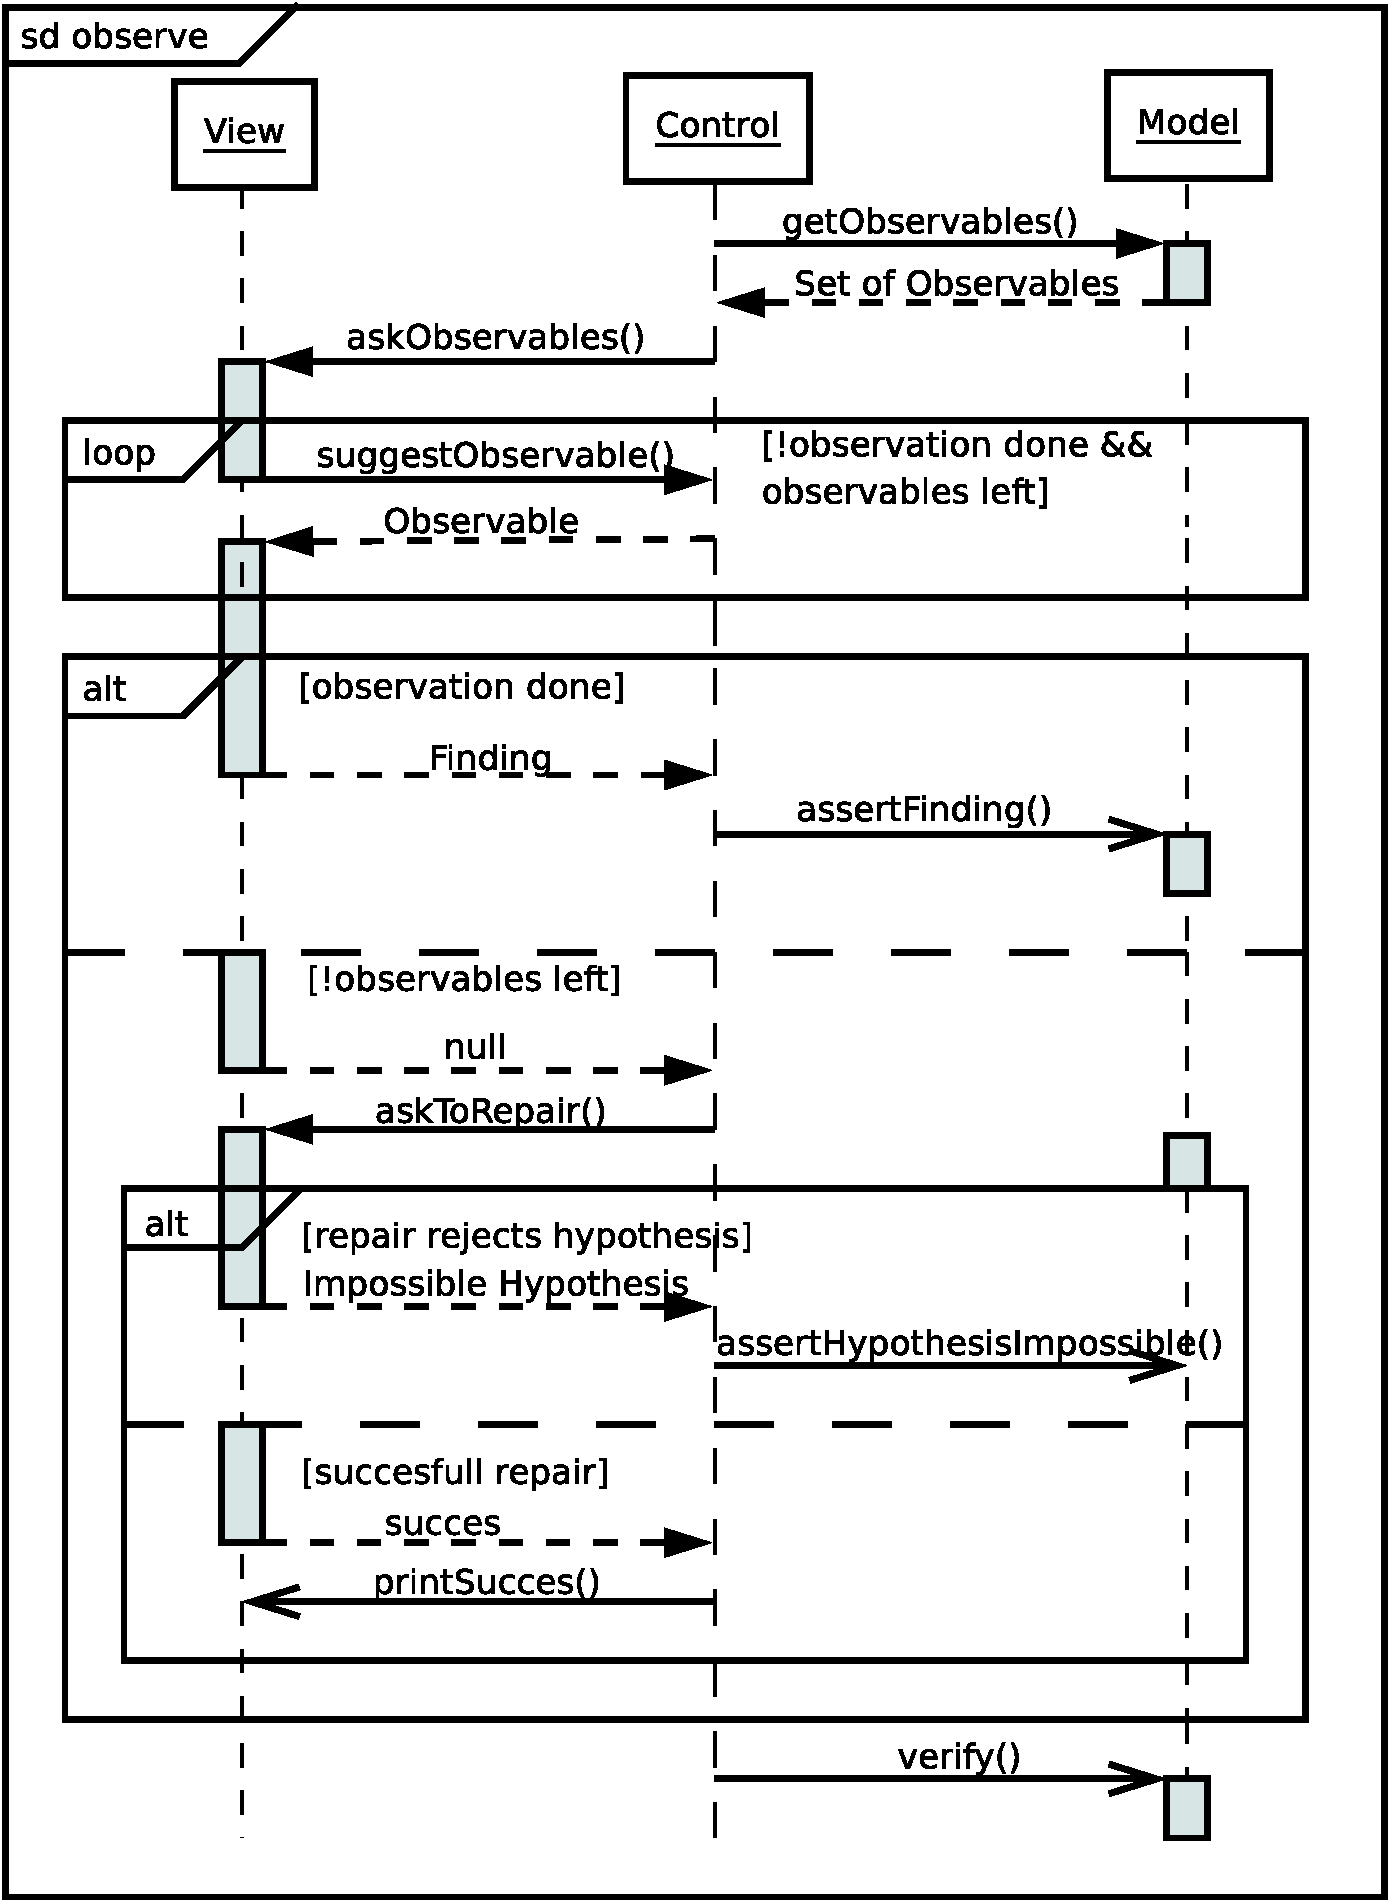
\includegraphics[width=1.00\textwidth]{dm-sd-observe}
    \caption{The state diagram detailing observations, try to repair and verify}
    \label{fig:dm:sd observe}
\end{figure}
